\documentclass[conference]{IEEEtran}
\IEEEoverridecommandlockouts
% The preceding line is only needed to identify funding in the first footnote. If that is unneeded, please comment it out.
% \usepackage{cite}
% Enables Portuguese Brasil
% \usepackage[portuguese]{babel}
%encoding
\usepackage[numbers]{natbib}
% Enables code listing
\usepackage{listings}
%--------------------------------------
\usepackage[T1]{fontenc}
\usepackage[utf8]{inputenc}
%--------------------------------------
%Enables the use of greek letter without a math context
\usepackage{textgreek}
%--------------------------------------
%Enables hiperlinks
\usepackage[hidelinks]{hyperref}
%--------------------------------------

\usepackage{amsmath,amssymb,amsfonts}
\usepackage{algorithmic}
\usepackage{graphicx}
\usepackage{textcomp}
\usepackage{xcolor}

\usepackage{color, colortbl}

% The code style
\usepackage{color}
\definecolor{codegreen}{rgb}{0,0.6,0}
\definecolor{codegray}{rgb}{0.5,0.5,0.5}
\definecolor{codepurple}{rgb}{0.58,0,0.82}
\definecolor{backcolour}{rgb}{0.95,0.95,0.92}

\lstdefinestyle{mystyle}{
	backgroundcolor=\color{backcolour},   
	commentstyle=\color{codegreen},
	keywordstyle=\color{magenta},
	numberstyle=\tiny\color{codegray},
	stringstyle=\color{codepurple},
	basicstyle=\footnotesize,
	breakatwhitespace=false,         
	breaklines=true,                 
	captionpos=b,                    
	keepspaces=true,                 
	numbers=left,                    
	numbersep=2pt,                  
	showspaces=false,                
	showstringspaces=false,
	showtabs=false,                  
	tabsize=2
}
\lstset{style=mystyle}
%---------------------------------------

\def\BibTeX{{\rm B\kern-.05em{\sc i\kern-.025em b}\kern-.08em
		T\kern-.1667em\lower.7ex\hbox{E}\kern-.125emX}}

\begin{document}
	\title{A tutorial of Solving the defined integral problem with OpenMp}
	\author{André Furlan - UNESP - Universidade Estadual Paulista "Júlio de Mesquita Filho"}
	\date{2023-06-01}
	\maketitle
	
	\begin{abstract}
		The Trapezoid rule algorithm used in this tutorial is \textbf{not} the most fast method to calculate an interval defined integral but is a good example of how to make programs runs quicker by using OpenMp for parallelism. Hopefully it will help the understanding of how this library works and how to use it. All sources can be accessed at \href{https://github.com/ensismoebius/ComputacaoDeAltoDesempenho}{https://github.com/ensismoebius/ComputacaoDeAltoDesempenho}
	\end{abstract}
	
	\begin{IEEEkeywords}
		OpenMp, Paralelism, C++, C, Tutorial
	\end{IEEEkeywords}
	
	\section{Introduction}
	\par In High Performance Computation (HPC) the goal (other than solve a problem) is to use most of the computation power of the machines involved. Most of the time this means use all processors an its cores at maximum, avoiding idle intervals.
	\par By using the OpenMp \cite{openmp08} libraries it is possible, using \textbf{\#pragma} compiler directives, turn a sequential program into a parallel one. The problem in focus here is the defined interval integral calculation. To solve it the program must calculate the area bellow the plot by summing up the area of several trapezoids \cite{hildebrand1987introduction}. The more trapezoids fitted, the more precise are the values obtained. And it is here that the parallelism enters: By dividing the work of area calculation in lots of threads its possible to diminish the effective time of execution.
	\section{The trapezoid rule}
	\par Be $a$ a point that marks the start of a interval in which the calculation must be done and $b$ its end, than an \textbf{approximation} of the integral value is given by equation \ref{eq:firstApproximation}. In figure \ref{fig:trapezoidalruleillustration} the basic idea is illustrated.\newline
	
	\begin{equation}
		\int^a_b{f(x) dx} \approx (b-a).\dfrac{1}{2}(f(a)+f(b))
		\label{eq:firstApproximation}
	\end{equation}

	\begin{figure}[h]
		\centering
		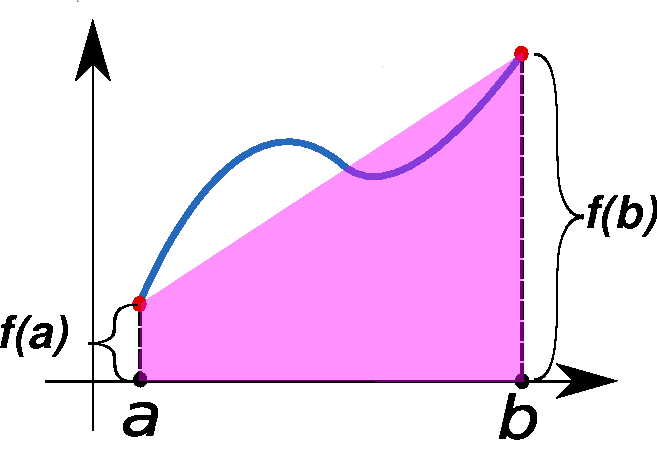
\includegraphics[width=0.7\linewidth]{images/Trapezoidal_rule_illustration}
		\caption[Approximation of an integral]{In pink the approximation(trapezoid area), in blue the actual function curve. $f(a)$ and $f(b)$ are the trapezoid bases and the interval $a, b$ its height. }
		\label{fig:trapezoidalruleillustration}
	\end{figure}
	
	\par The figure \ref{fig:trapezoidalruleillustration} and the equation \ref{eq:firstApproximation} shows a pretty coarse approximation! What if the $[a, b]$ interval get subdivided (partitioned) like in figure \ref{fig:trapezoidalruleillustration2}? Well, then it is possible to get a value closer to the real one!\newline
	
	\begin{figure}[h]
		\centering
		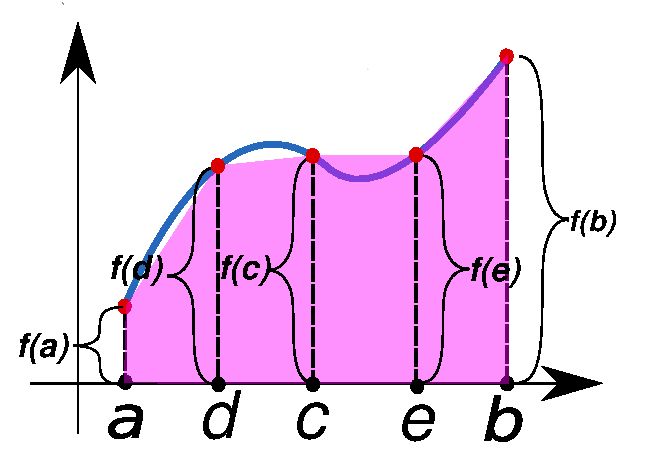
\includegraphics[width=0.7\linewidth]{images/Trapezoidal_rule_illustration2}
		\caption[Enhanced approximation of an integral]{In pink the \textbf{enhanced} approximation(trapezoid area), in blue the actual function curve. $f(a), f(b), f(c), f(d), f(e)$ are the trapezoid bases and the intervals $[a, d],[d,c], [c,e], [e,b]$ its heights. Note that now there are 4 trapezoids i.e. 4 areas that must be calculated. }
		\label{fig:trapezoidalruleillustration2}
	\end{figure}

	\par To obtain the result all areas must be summed up, therefore the equation \ref{eq:firstApproximation} turns into \ref{eq:secondApproximation}. So, as many partitions are made, the more sums are added.\newline
	
	\begin{equation}
		\begin{aligned}
			\int^a_b{f(x) dx} \approx 
			&(d-a).\dfrac{1}{2}(f(d)+f(a))+\\
			&(c-d).\dfrac{1}{2}(f(c)+f(d))+\\
			&(e-c).\dfrac{1}{2}(f(e)+f(c))+\\
			&(b-e).\dfrac{1}{2}(f(b)+f(e))
		\end{aligned}
		\label{eq:secondApproximation}
	\end{equation}

	\par Let $x = [a,b]$ and $n=partitions+1=points$ of $[a,b]$ than it is true to say that $x_0 = a < x_1 < ... < x_{n-1} < x_n = b$. Being the interval between two points $\Delta_{x_k} = x_k - x_{k-1}$ than the equation \ref*{eq:secondApproximation} can be rewrote as in the equation \ref{eq:genericApproximation}.\newline
	
	\begin{equation}
		\int^a_b{f(x) dx} \approx \sum_{k=1}^{n} \dfrac{f(x_{k-1})+f(x_k)}{2} . \Delta_{x_k}
		\label{eq:genericApproximation}
	\end{equation}

	\par And this is (finally) the idea that will be implemented ahead!
	
	\section{Implementation}
		\par First of all it is necessary to define a function to integrate, the one used here is defined in equation \ref{eq:function} and the integration interval begins in \textbf{0 until 100}. The performance will be tested using \textbf{1, 2, 4 and 8 threads}.  Note that this method supports any function, this one was chosen for example purposes only.\newline
		
		\begin{equation}
			f(x) = \sqrt{100^2 - x^2}
			\label{eq:function}
		\end{equation}		
		
		\par Then, for the impatient ones, here is the complete code that will be discussed:
		\lstinputlisting[language=C++]{code/integral.cpp}
			
	\section{Discussion}
		\par This section focus only in the OpenMp directives, its assumed that the reader knows a minimum of C++.\newline
		
		\par The lines 5 to 7 includes OpenMp header files if the build system used detected such library.
		\begin{lstlisting}[language=C++]
#ifdef _OPENMP
	#include <omp.h>
#endif
		\end{lstlisting}
	
		\par From line 9 to 12, the function to be integrated is defined. Note the \textit{inline} statement: Inlinning functions \textbf{may} avoid the intrinsic overhead of calling a function but, since this it is not a command, the compiler may ignore this request.
		\begin{lstlisting}[language=C++]
inline long double f(long double x)
{
	return std::sqrt(std::pow(100,2) - std::pow(x,2));
}
		\end{lstlisting}
		
		\par Line 22 states that the variable \textit{sum} is shared by all threads all the other variables are not.
		\begin{lstlisting}[language=C++]
#pragma default(none) shared(soma)
		\end{lstlisting}
		
		\par At the 24 position OpenMp starts a parallel zone: From now on the instructions are replicated in several  threads according to parallelization rules defined in the \textbf{operational system ambient variables} \cite{openmp08SV}. The zones are defined using curling braces (same as blocks in C++).
		\begin{lstlisting}[language=C++]
#pragma omp parallel
		\end{lstlisting}
	
		\par The most important part is declared here in line 26. This directive is the heart of the parallelization for this algorithm. For each thread \textit{sum} is initialized to 0 then, after all calculations, the obtained values are summed together. For this directive it have to be possible to known beforehand the number of iterations in execution time i.e. the number of iterations cannot change while the loop are being executed. Also the k variable (used in for loop) must \textbf{not} be modified within the loop otherwise it can be changed like in k++ statement. Since, in this specific case, a summation is need OpenMp have a convenient \textit{reduction} directive that enables it. The \textit{reduction} directive can be used with other types of operations like \textit{subtractions}, \textit{maximums} and \textit{minimums}. 
		
		\begin{lstlisting}[language=C++]
#pragma omp for reduction(+ : sum)
		\end{lstlisting}
	
		\par Finally, at the line 31, a barrier to the execution of the program is created in order to ensure that all threads has been finished until this point. Now it is possible to do another operations with the outputted sum.  This is optional in this \textbf{specific case} because there is an implicit barrier in \textit{for} directive. It is important to note that \textbf{there is no code} associated with this directive i.e. it just marks a point where all threads must arrive. \textbf{Warning!} All or none of the threads must encounter the barrier otherwise a \textbf{deadlock} happens.
		
		\begin{lstlisting}[language=C++]
#pragma omp barrier
		\end{lstlisting}
	
		\par Among the aforementioned \textbf{operational system ambient variables} one is the most important for the sake of this program: OMP\_NUM\_THREADS. This variable sets the number of threads (an integer) that are going to be used when running the algorithm. If no value is assigned than the maximum of threads supported are used.

	\section{Performance tests}
		\par The tests were done using an \textit{AMD Ryzen 5 5000 series} processor running an \textit{Gnu/Linux operational system} with \textit{30GB of RAM}.\newline
		
		\par The tables bellow shows the results according to the number of threads. 
		
		\begin{table}[h]
			\caption{export OMP\_NUM\_THREADS=1}
			\begin{center}
				\begin{tabular}{|l|l|l|l|}
					\hline
					Interval $\Delta_{x_k}$  &  Partitions  &  Time taken in sec &  Result \\
					\hline
					0.000001  &  100000000  &  0.670965  &  7853.981634 \\
					\hline
					0.000010  &  10000000  &  0.067101  &  7853.981633 \\
					\hline
					0.000100  &  1000000  &  0.006715  &  7853.981617 \\
					\hline
				\end{tabular}
			\end{center}
		\end{table}
		
		\begin{table}[h]
			\caption{export OMP\_NUM\_THREADS=2}
			\begin{center}
				\begin{tabular}{|l|l|l|l|}
					\hline
					Interval $\Delta_{x_k}$  &  Partitions  &  Time taken in sec &  Result \\
					\hline
					0.000001  &  100000000  &  0.341421  &  7853.981634 \\
					\hline
					0.000010  &  10000000  &  0.033588  &  7853.981633 \\
					\hline
					0.000100  &  1000000  &  0.003378  &  7853.981617 \\
					\hline
				\end{tabular}
			\end{center}
		\end{table}
		
		\begin{table}[h]
			\caption{export OMP\_NUM\_THREADS=4}
			\begin{center}
				\begin{tabular}{|l|l|l|l|}
					\hline
					Interval $\Delta_{x_k}$  &  Partitions  &  Time taken in sec &  Result \\
					\hline
					0.000001  &  100000000  &  0.172951  &  7853.981634 \\
					\hline
					0.000010  &  10000000  &  0.016810  &  7853.981633 \\
					\hline
					0.000100  &  1000000  &  0.001684  &  7853.981617 \\
					\hline
				\end{tabular}
			\end{center}
		\end{table}
			
		\begin{table}[h]
			\caption{export OMP\_NUM\_THREADS=8}
			\begin{center}
				\begin{tabular}{|l|l|l|l|}
					\hline
					Interval $\Delta_{x_k}$  &  Partitions  &  Time taken in sec &  Result \\
					\hline
					0.000001  &  100000000  &  0.144975  &  7853.981634 \\
					\hline
					0.000010  &  10000000  &  0.014428  &  7853.981633 \\
					\hline
					0.000100  &  1000000  &  0.001436  &  7853.981617 \\
					\hline
				\end{tabular}
			\end{center}
		\end{table}
	
	\section{Conclusion}
	\par Conclusion
	
	\bibliographystyle{plain}
	\bibliography{references.bib}
\end{document}